\section{Analysis and results}
\label{sec:analysis}

\subsection{Calibration of PS scintillator}
\label{sub:calibration}
The purpose of this section is to calibrate the channels to known energies, in our case
\begin{itemize}
\item $^{22}$Na Compton edge 1: 341 keV
\item $^{22}$Na Compton edge 2: 1064 keV
\item $^{137}$Cs Compton edge: 477 keV
\end{itemize}
First we fitted the two Compton edges of the $^{22}$Na sample, the result is
Channel $108 \pm 2$ and $414 \pm 4$ with a correlation of about 50\%, see
figure~\ref{fig:calib_ps_na}.

\begin{figure}[htpb]
    \centering
    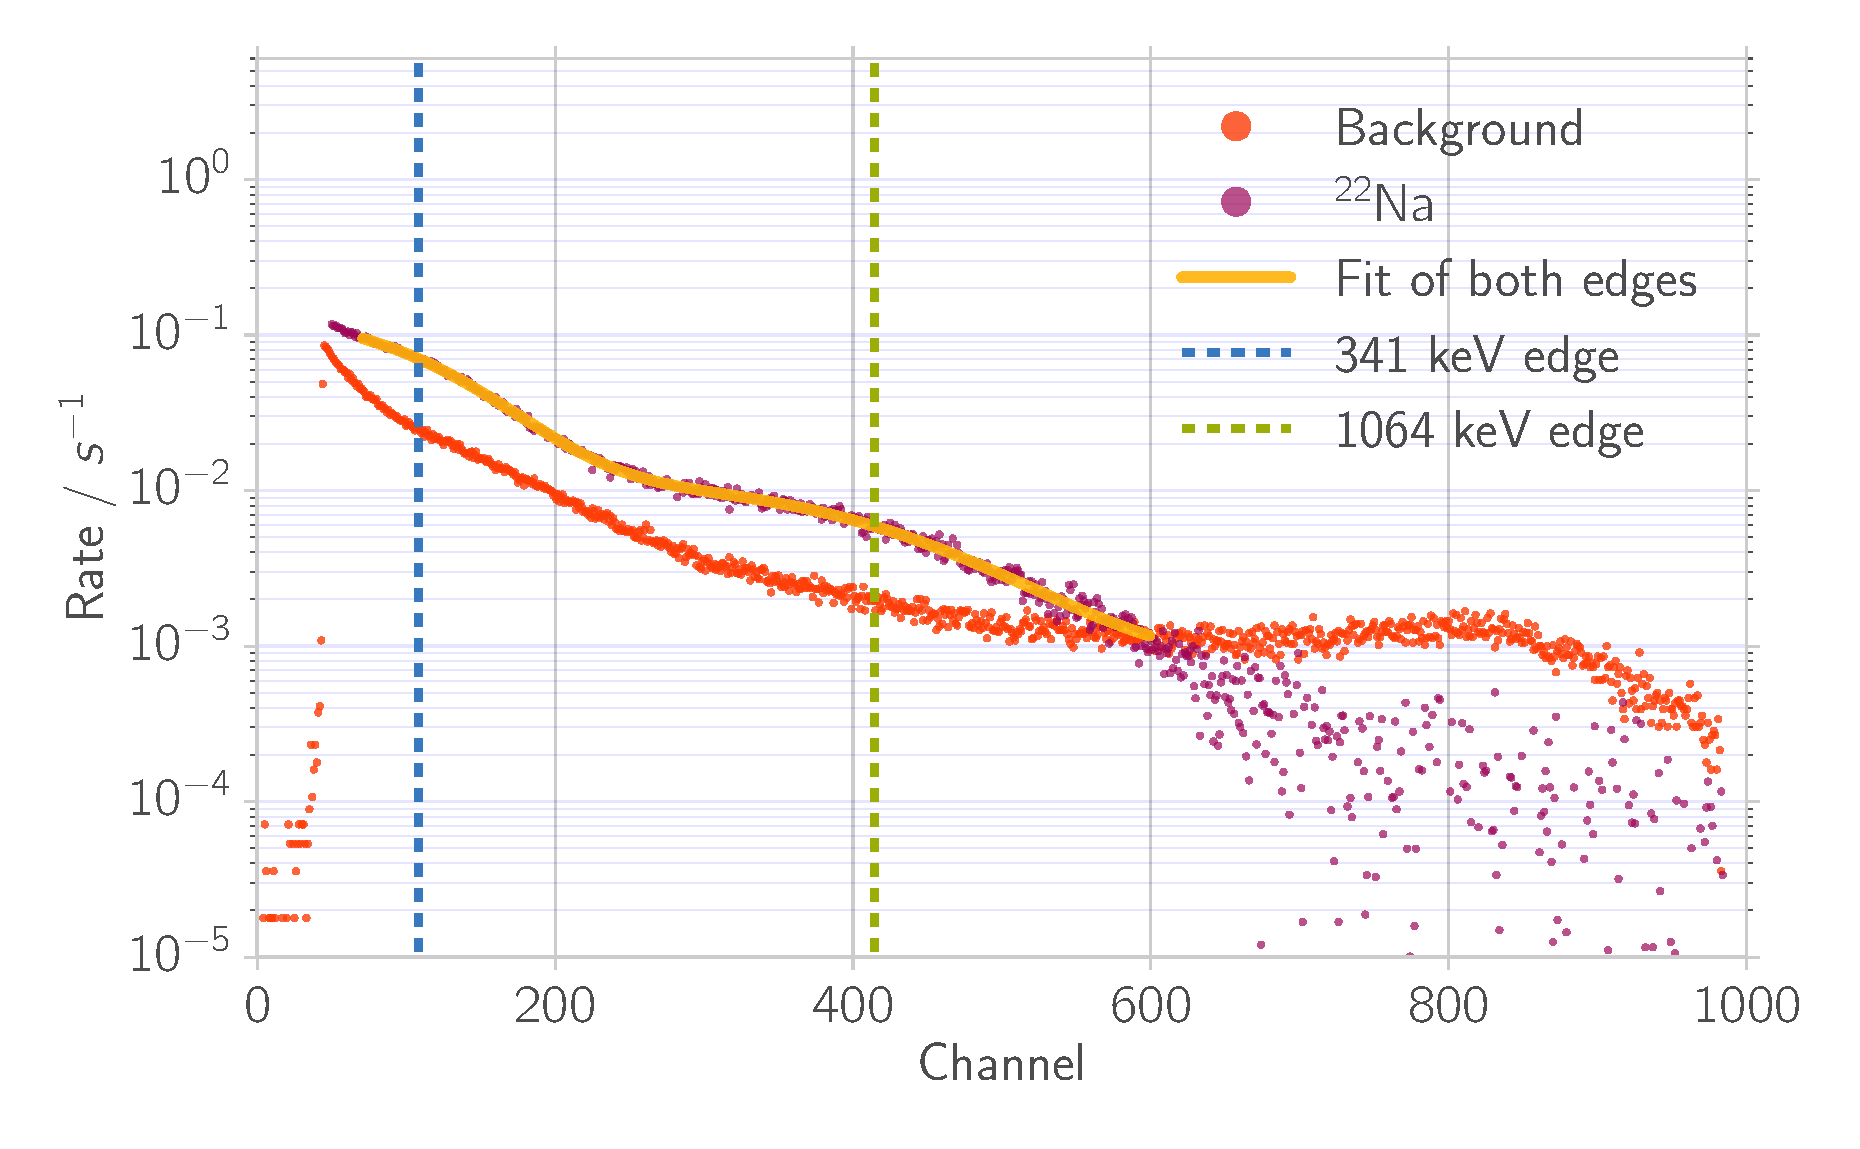
\includegraphics[width=0.9\linewidth]{./analysis/figures/calib_ps_na}
    \caption{Calibration of the PS scintillator with $^{22}$Na sample (measurement time
    16.5 h) with refined background (measurement time 15.6h). As you can notice, rate is 
only fitted for the section in which the background is smaller than the sample. We
subtracted the background rate at each channel for the sample in order not to fit the 
behavior of the noise. The error of the two Compton edges is large (see text) coming
from the fit and their high correlation coefficient.}
\label{fig:calib_ps_na}
\end{figure}
For the $^{137}$ sample we found the Compton at Channel $178.9 \pm 0.3$ 
(notice the much smaller error compared to the $^{22}$Na sample), 
see figure~\ref{fig:calib_ps_cs} for the data and the fit.
\begin{figure}[htpb]
    \centering
    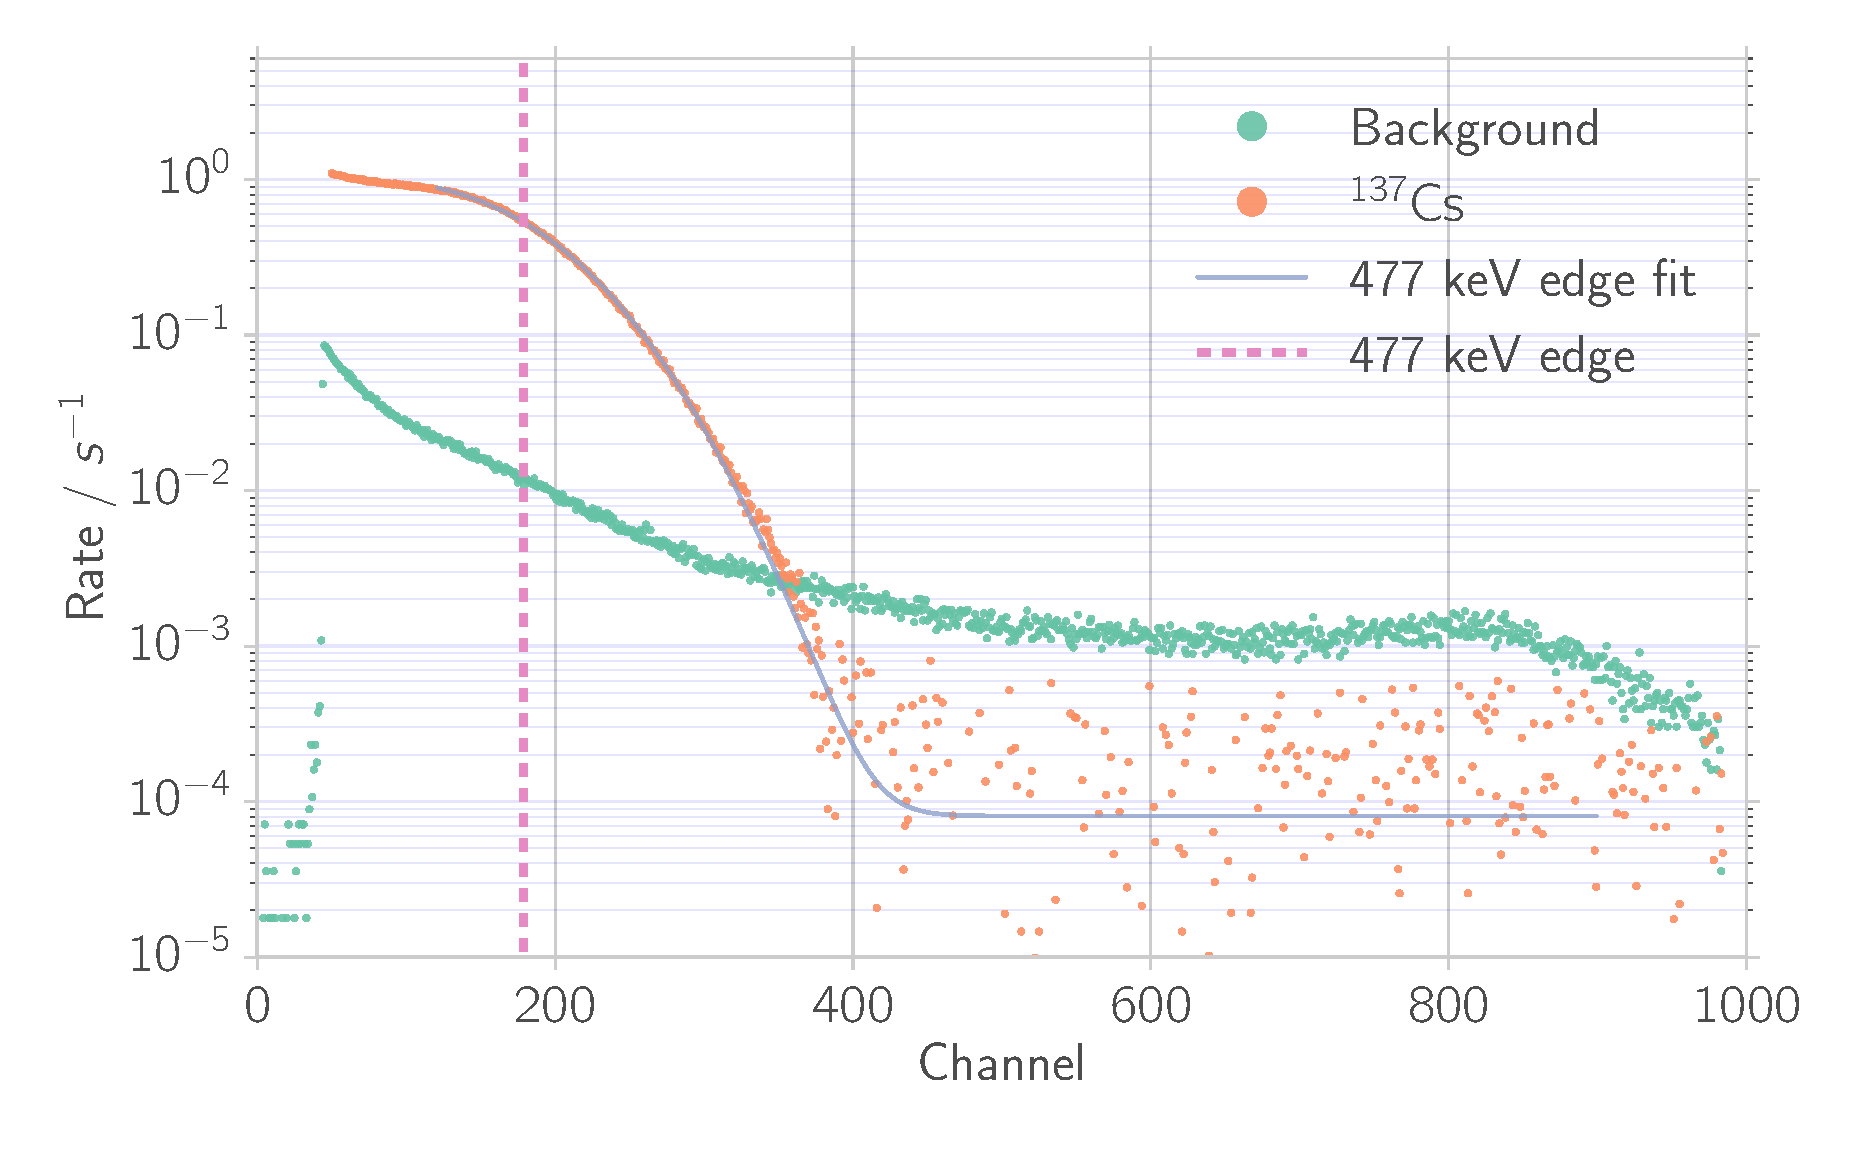
\includegraphics[width=0.9\linewidth]{./analysis/figures/calib_ps_cs}
    \caption{Calibration of the PS scintillator, same as figure~\ref{fig:calib_ps_na}. 
        with $^{137}$Cs sample (measurement time
    6 h) with refined background (measurement time 15.6h, same as before). 
Again we subtracted the background rate at each channel behavior of the noise. }
\label{fig:calib_ps_cs}
\end{figure}

\begin{figure}[htpb]
    \centering
    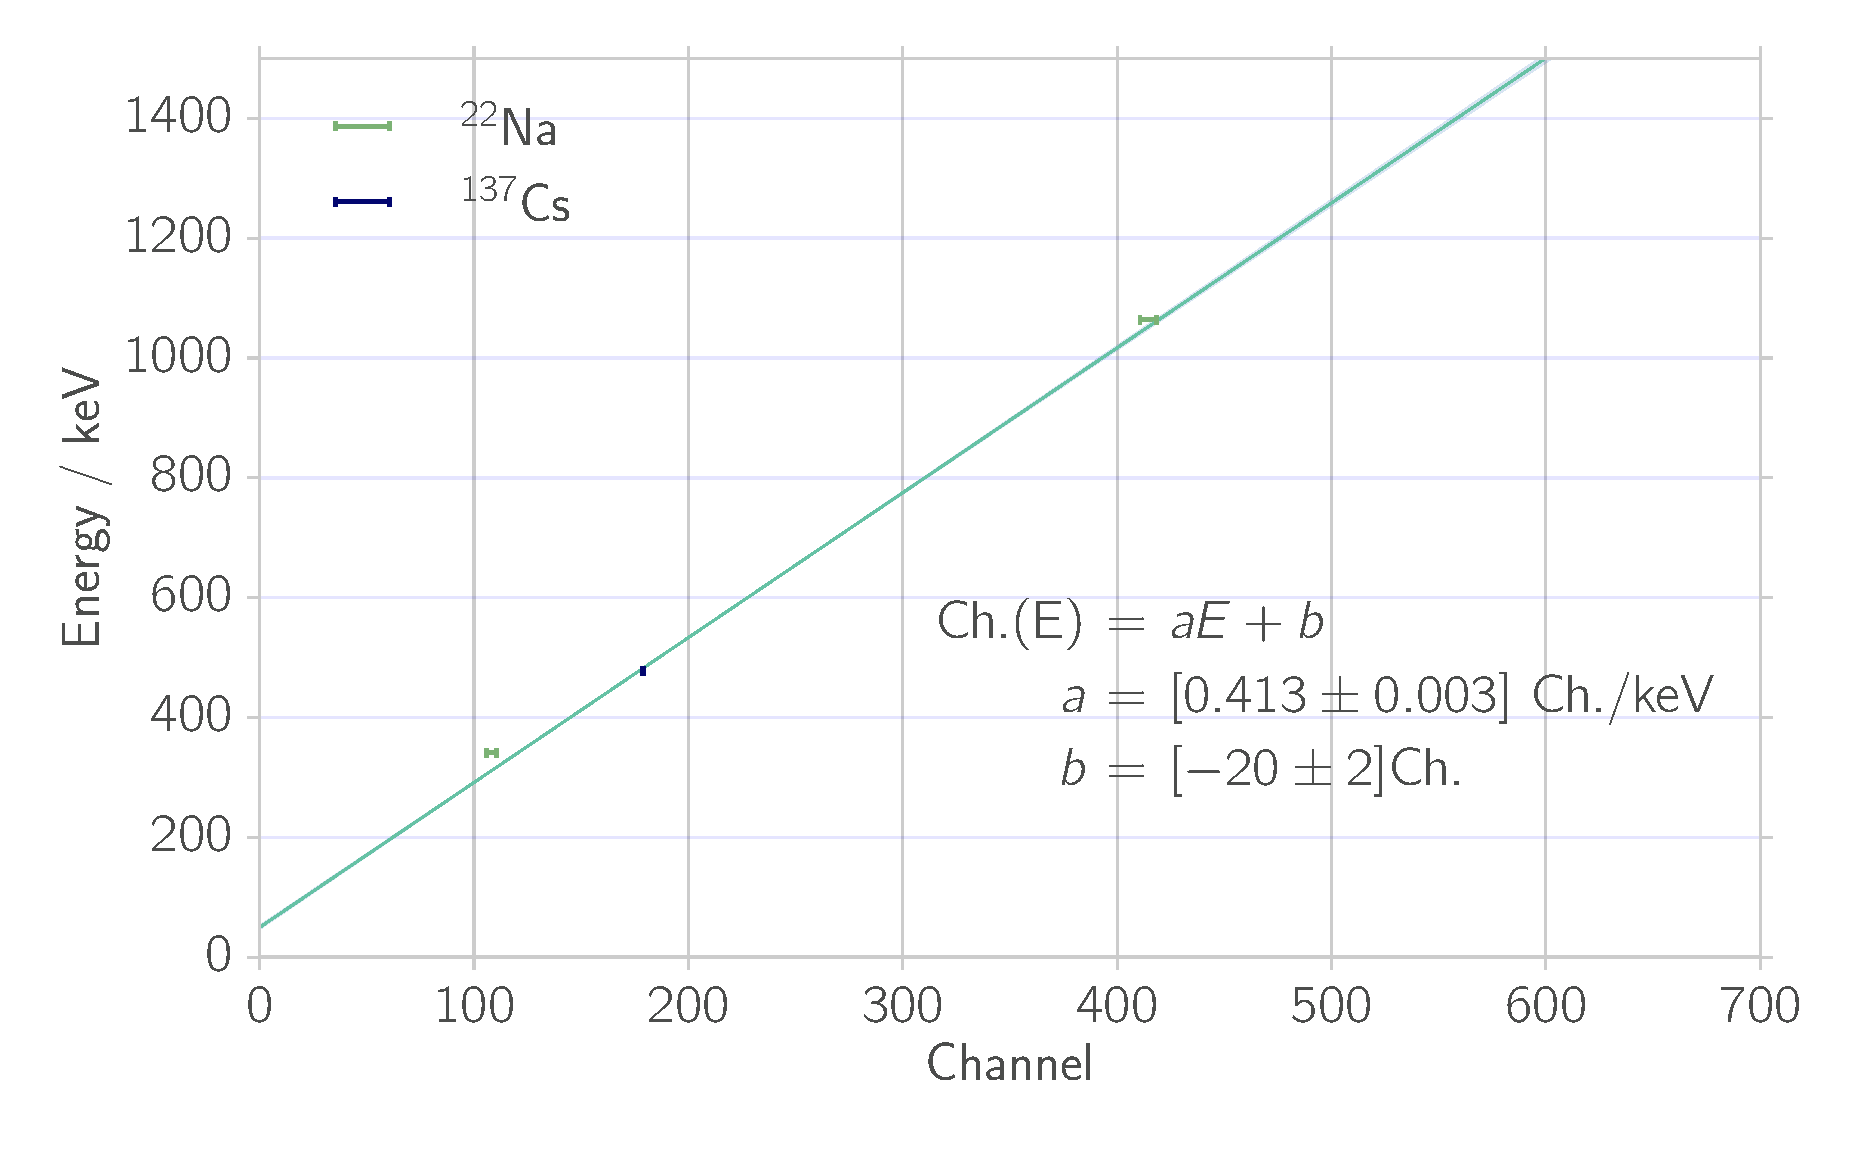
\includegraphics[width=0.9\linewidth]{./analysis/figures/calibration_ps_linear_fit}
    \caption{This is the result of the three Compton edges. We will use this calibration
    for all the following calculations.}
\label{fig:calibration_ps_linear_fit}
\end{figure}
The final result of the linear calibration can be seen in
figure~\ref{fig:calibration_ps_linear_fit}.

\subsection{Calibration of Na scintillator}

\label{sub:calibration_of_na_scintillator}
As in the last section we find a calibration now, this time for the Na scintillator. The
first figure~\ref{fig:histo_na_137cs} shows the $^{136}$Cs sample where we know the
peaks from the literature, see table~\ref{tab:peaks_cs_ps}, whereas the data for
$^{22}Na$ can be seen in figure~\ref{fig:histo_na_22na} and figure~\ref{fig:histo_na_22na2}
and the results are summarized in table table~\ref{tab:peaks_na_ps}. 
The final result of the linear calibration can be seen in
fig~\ref{fig:calibration_na_linear_fit}.
\begin{table}[htpb]
    \centering
    \caption{Peaks and fitting results of $^{136}$Cs.}
\label{tab:peaks_cs_ps}
    \begin{tabular}{lll}
        \rowcolor{LightCyan} Name &Energy & Channel \\ 
        Photo peak & 662 keV & $8040.59 \pm 0.03$\\ 
        Compton edge & 477 keV & $5720 \pm 4$\\  
        Escape peak & 183 keV & $2510 \pm 12$
    \end{tabular}
\end{table}

\begin{figure}[htpb]
    \centering
    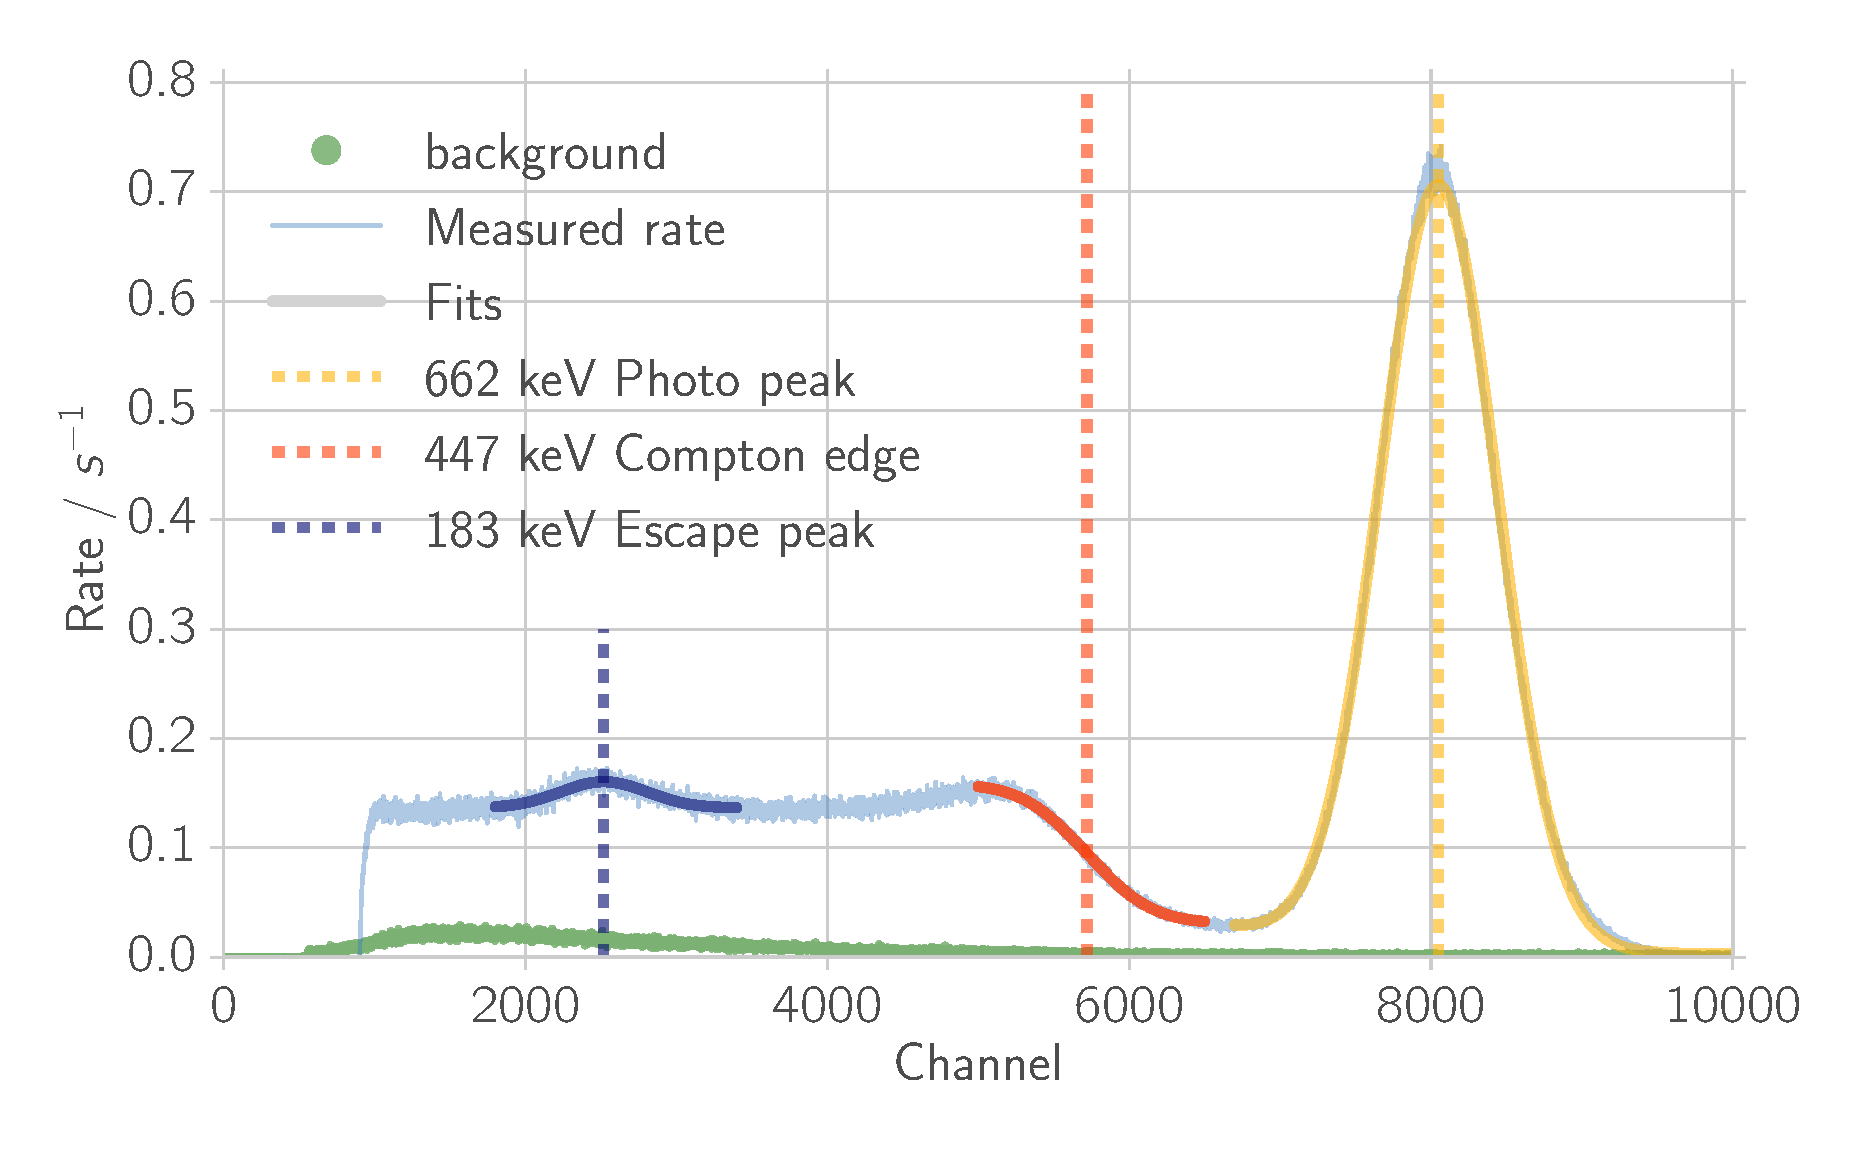
\includegraphics[width=0.9\linewidth]{./analysis/figures/histo_na_137cs}
    \caption{Calibration of the Na scintillator using $^{137}$Cs sample (measurement
    time 2.7h) with refined background (measurement time 1h). }
\label{fig:histo_na_137cs}
\end{figure}

\begin{figure}[htpb]
    \centering
    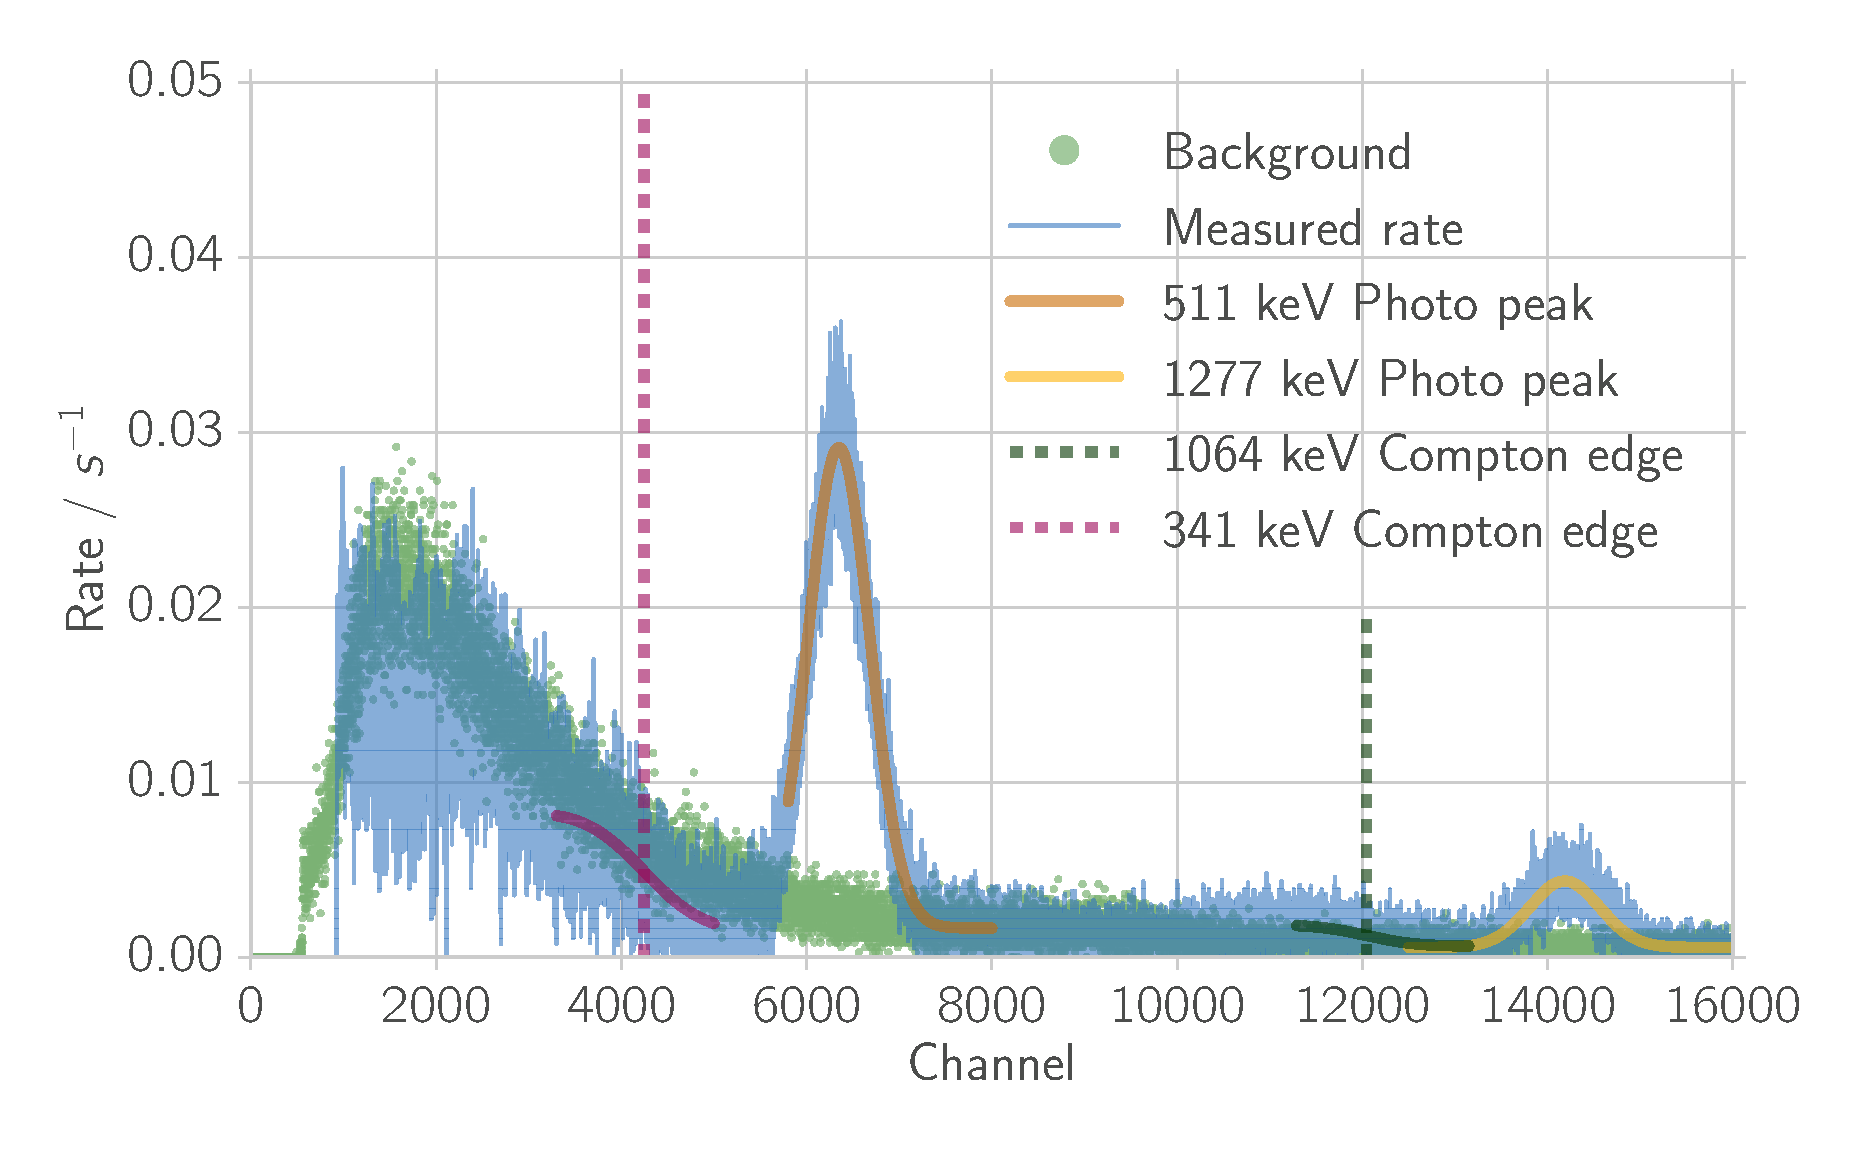
\includegraphics[width=0.9\linewidth]{./analysis/figures/histo_na_22na}
    \caption{Calibration of the Na scintillator using $^{22}$Na sample (measurement
        time about 1h) with refined background (same as in figure~\ref{fig:histo_na_137cs},
        measurement time 1h). }
\label{fig:histo_na_22na}
\end{figure}

\begin{figure}[htpb]
    \centering
    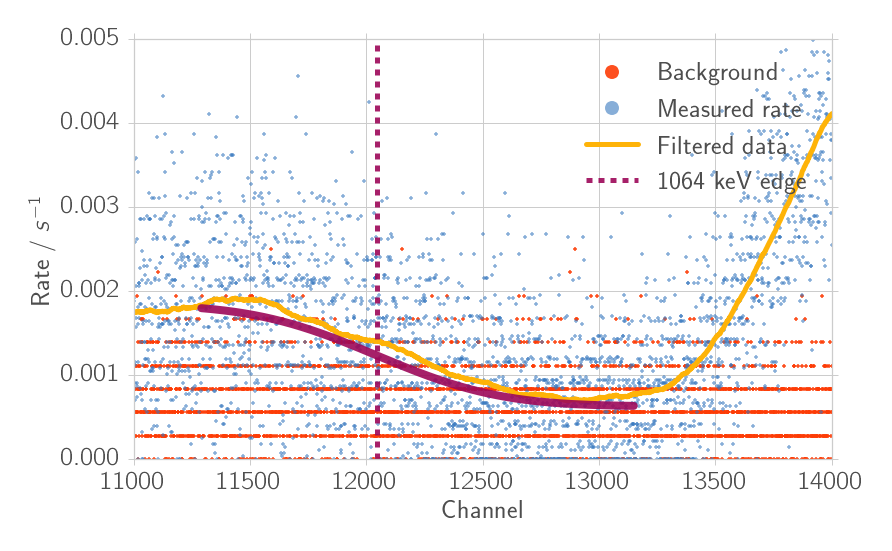
\includegraphics[width=0.9\linewidth]{./analysis/figures/histo_na_22na2}
    \caption{Enlargement of the critical area of the Compton edge of
    figure~\ref{fig:histo_na_22na}.     
    The red line is a Savitzky-Golay filter 
    with a width of 1001 points and a fourth
    degree polynomial applied to the data (see~\cite{scipy} for reference) in order
    to see the slope of the curve. The least-squares fit uses the real data, though.
}
\label{fig:histo_na_22na2}
\end{figure}

\begin{table}[htpb]
    \centering
    \caption{Peaks and fitting results of $^{22}$Na. As it is also visible in the figure
    of the leasts-squares fit~\ref{fig:calibration_na_linear_fit} the errors on the
    Compton edges are much higher than those of the Photo peaks. This is due to the high
    degree of uncertainty of the particular edge resulting from the fit. However, the 
    uncertainty of the linear fit is much less in the end.}
\label{tab:peaks_na_ps}
\begin{tabular}{lll}
    \rowcolor{LightCyan} Name &Energy & Channel \\ 
       1. Photo peak& 511 keV & $6347 \pm 3$ \\ 
       2. Photo peak& 1277 keV & $14180 \pm 20 $\\
       1. Compton edge& 341 keV& $4000 \pm 2000$\\
       2. Compton edge& 1064 keV & $12000 \pm 4000$
    \end{tabular}
\end{table}

\begin{figure}[htpb]
    \centering
    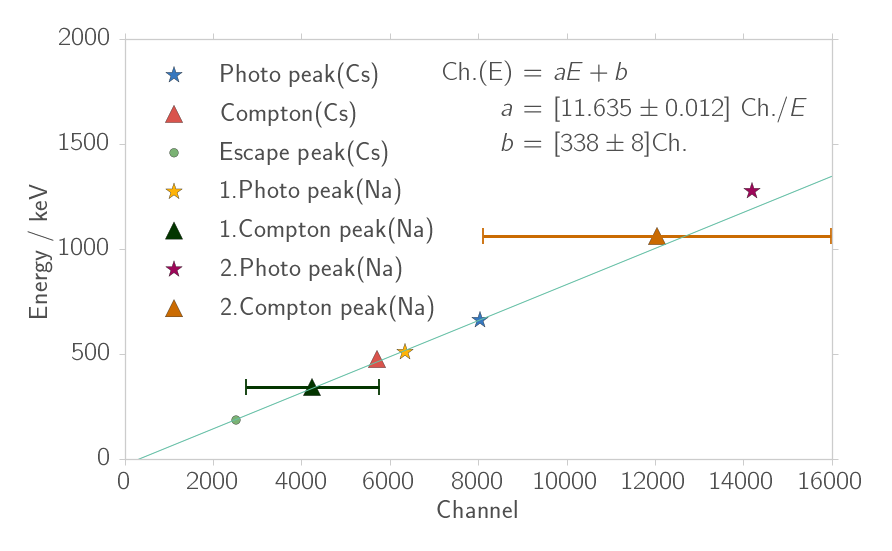
\includegraphics[width=0.9\linewidth]{./analysis/figures/calibration_na_linear_fit}
    \caption{All peaks in one figure with the respective linear fit. The errors of
    the most of the peaks are too small to be shown, only the Compton peaks of Na show
    an exorbitant error. The second Photo peak (Na Sample) seems to be quite apart from
    the result of the other values; this might be due to a general systematic error.}
\label{fig:calibration_na_linear_fit}
\end{figure}
\clearpage
\subsection{Energy conservation}
\label{sub:energy_conservation}
In this section we work out the dependence of the energy with respect to the scattered
angle. Figure~\ref{fig:coin_ps_background} shows the background (with
coincident setup but without sample and with random coincidences of the sample).
As always, we subtract the background from our data before pursuing the analysis.
This will include evaluating a number of different measurements; we will
only show two example figures for each detector 
(figures~\ref{fig:coin_ps_90} and~\ref{fig:coin_ps_15} for the PS scintillator and 
~\ref{fig:coin_na_90} and~\ref{fig:coin_na_30} for the Na scintillator). The main
result is summarized in figure~\ref{fig:coin_na_90}, it shows the expectation values of
the energy, dependent on different scattering angles $\theta$.


\begin{figure}[htpb]
    \centering
    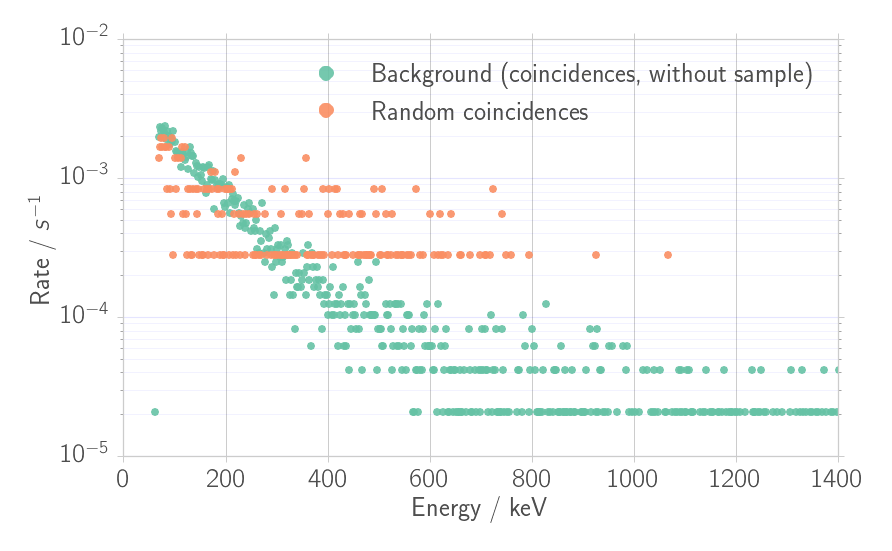
\includegraphics[width=0.9\linewidth]{./analysis/figures/coin_background_random}
    \caption{This is the background of the PS scintillator with coincidence
        (measurement time 13.4h)  
 and with random coincidences (measurement time 1h).}
\label{fig:coin_ps_background}
\end{figure}

\begin{figure}[htpb]
    \centering
    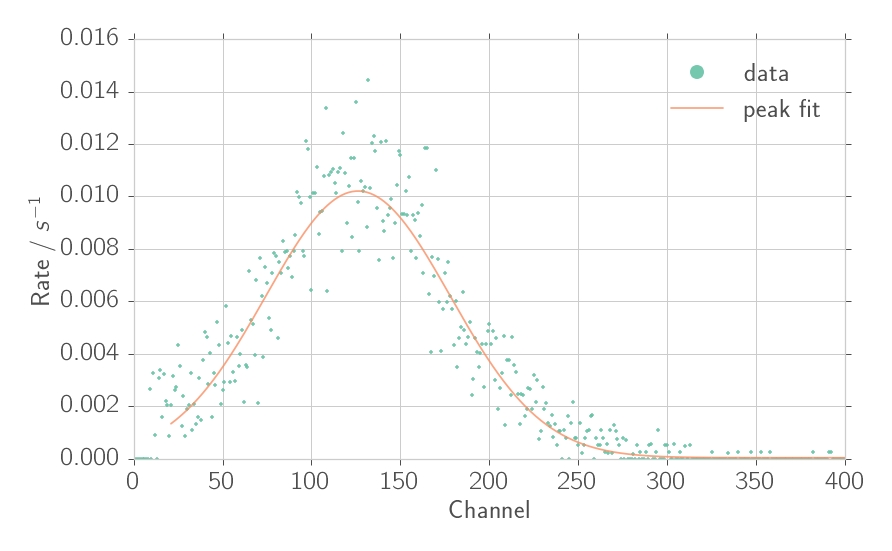
\includegraphics[width=0.9\linewidth]{./analysis/figures/coin_ps_90}
    \caption{\textbf{Energy of electrons:}
    Rate of coincident events of PS scintillator at angle of $\theta = 90^\circ$ 
        (measurement time between 30min and 1h). The distribution 
    was approximated with a Gaussian distribution. }
\label{fig:coin_ps_90}
\end{figure}

\begin{figure}[htpb]
    \centering
    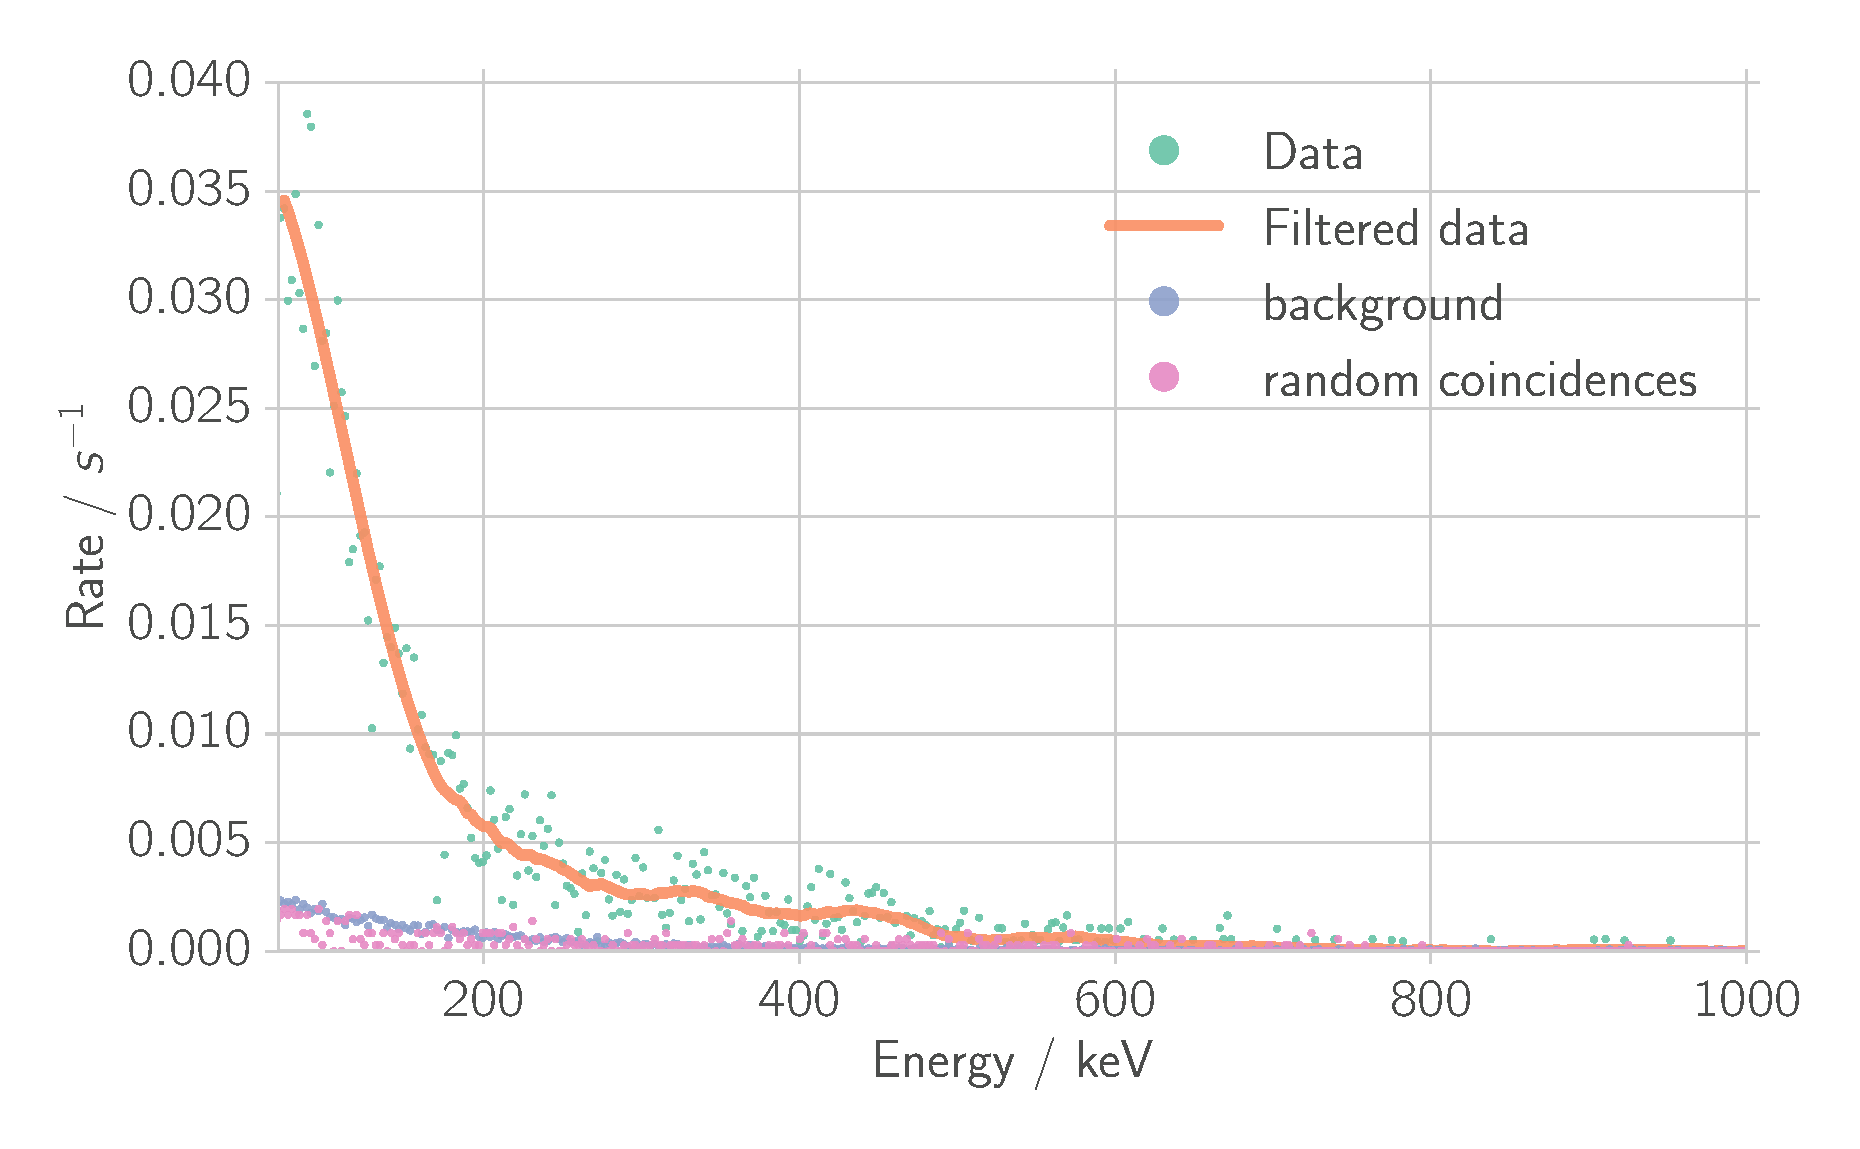
\includegraphics[width=0.9\linewidth]{./analysis/figures/coin_ps_15_filter_}
    \caption{\textbf{Energy of electrons:}
        Rate of coincident events of 
        PS scintillator at angle of $\theta = 15^\circ$.
        In this figure we used, unlike at higher angles, applying the Savitzky-Golay filter
        with a width of 81 points and a fourth
    degree polynomial (see~\cite{scipy} for reference). This was done for 
angles $\theta = 15^\circ$ up to $\theta = 60^\circ$.}
\label{fig:coin_ps_15}
\end{figure}

\begin{figure}[htpb]
    \centering
    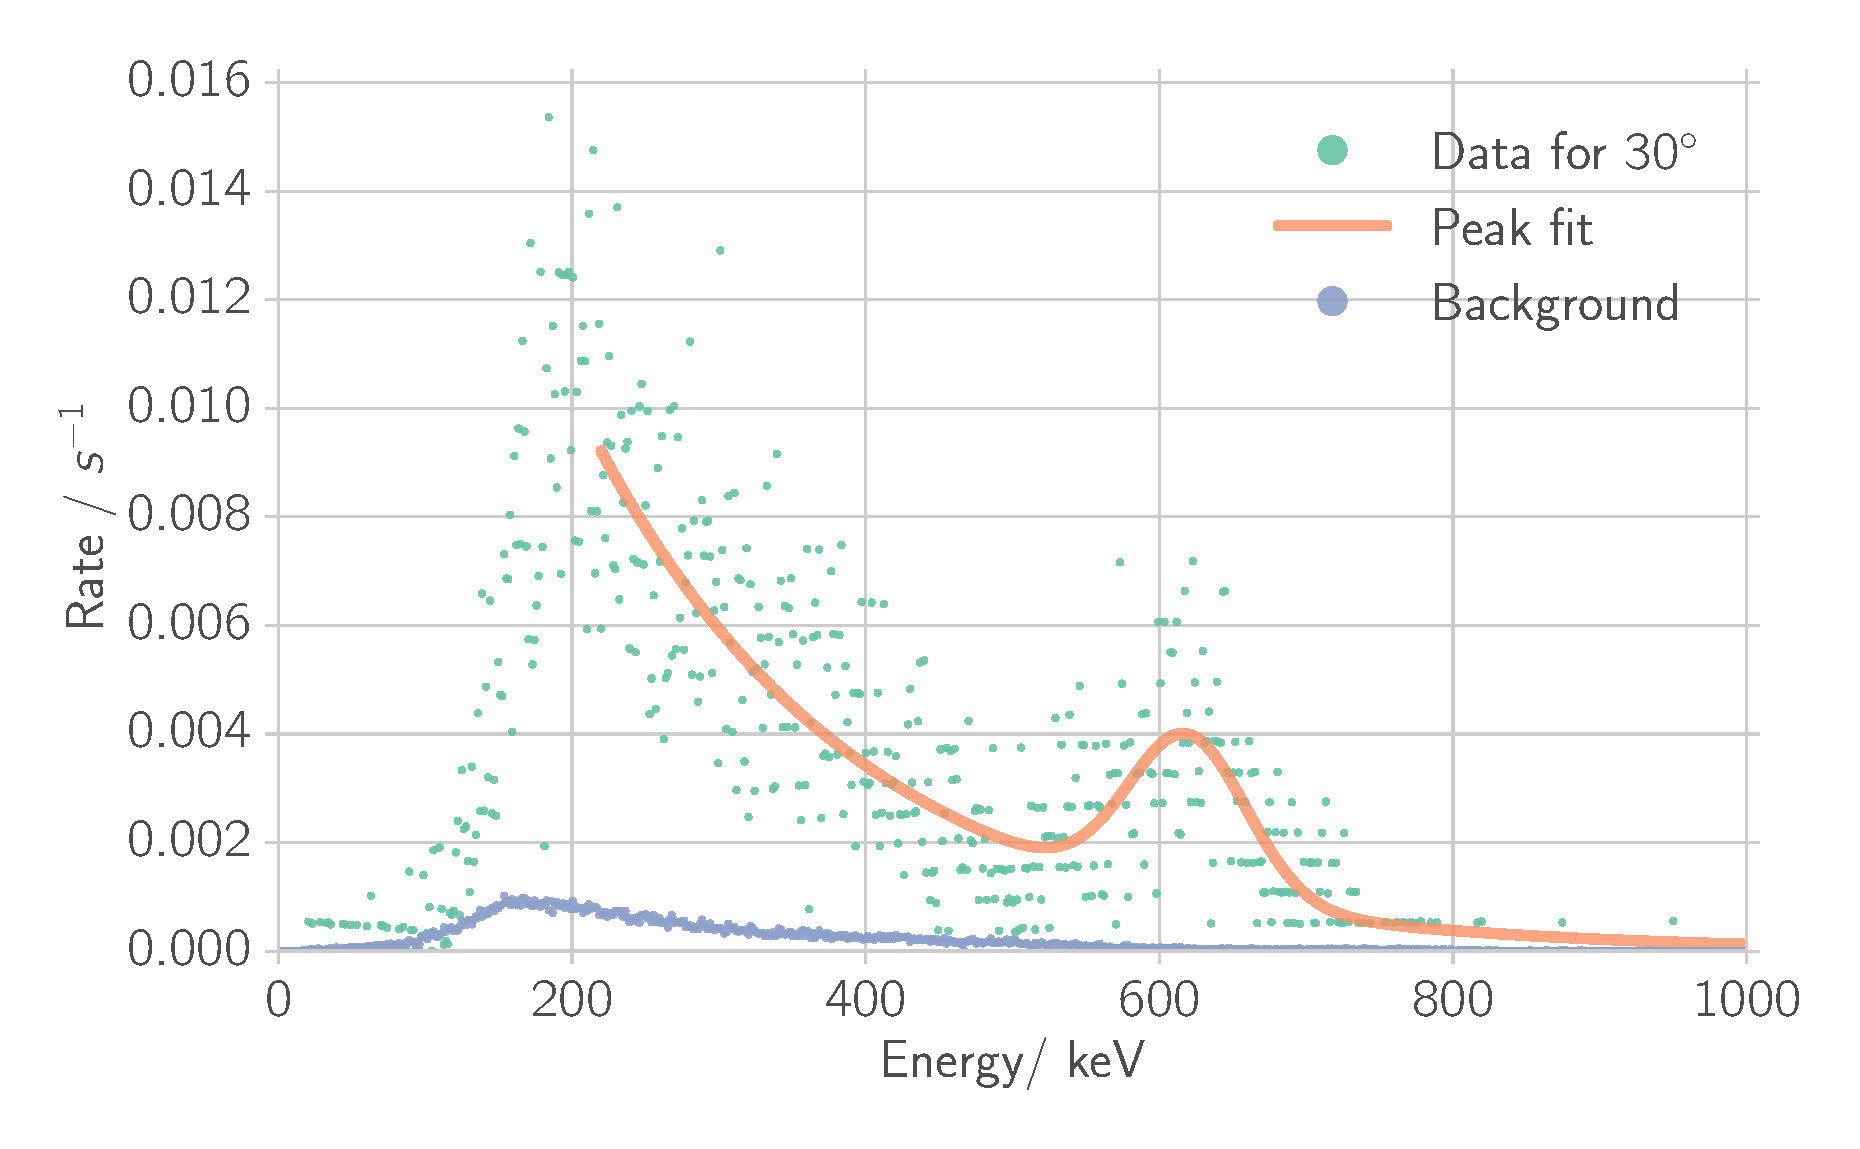
\includegraphics[width=0.9\linewidth]{./analysis/figures/coin_na_30}
    \caption{\textbf{Energy of photons:} Rate of coincident events of 
        Na scintillator at angle of $\theta = 15^\circ$. The Photo peak was approximated
    with a Gaussian distribution.}
\label{fig:coin_na_30}
\end{figure}




\begin{figure}[htpb]
    \centering
    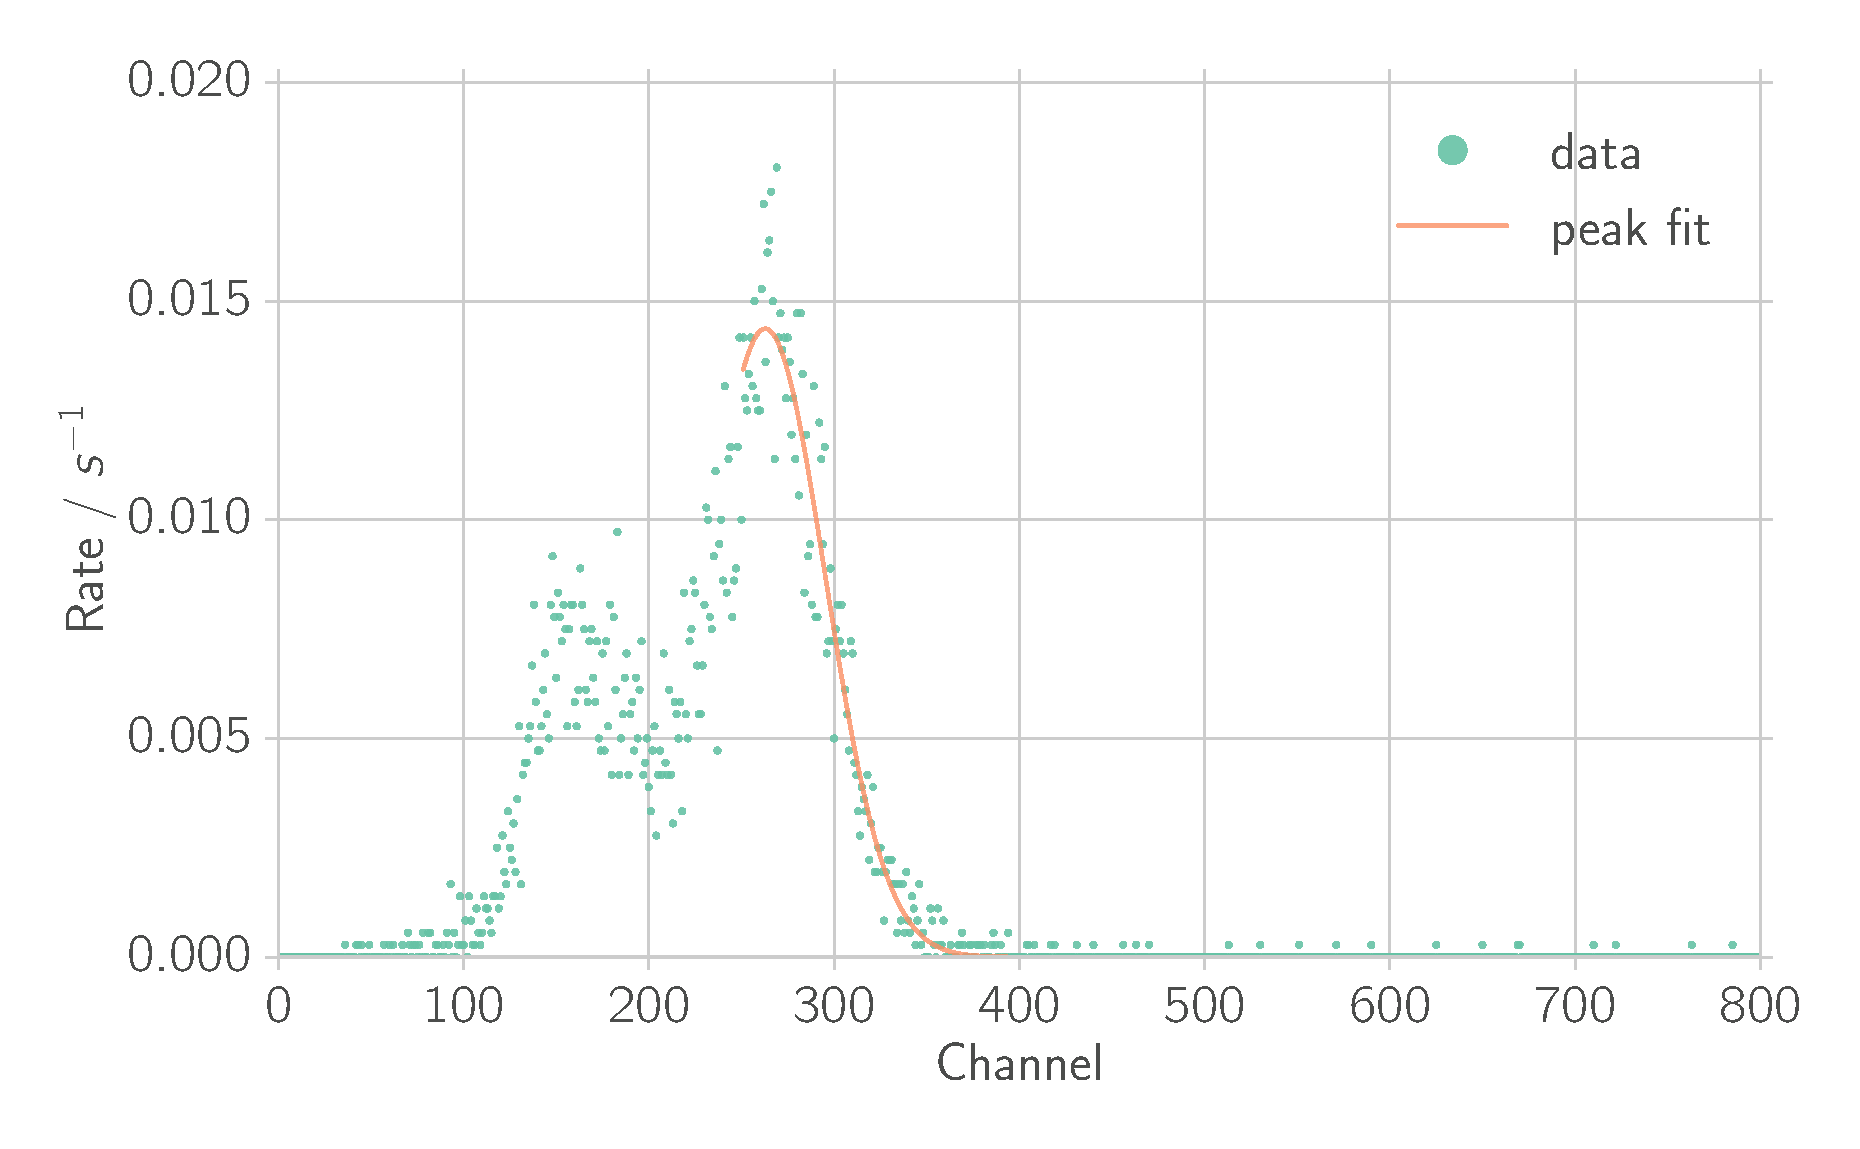
\includegraphics[width=0.9\linewidth]{./analysis/figures/coin_na_90}
\caption{\textbf{Energy of photons:} Rate of coincident events of 
        Na scintillator at angle of $\theta = 90^\circ$. The distribution 
    was approximated with a Gaussian distribution. }
\label{fig:coin_na_90}
\end{figure}


\begin{figure}[htpb]
    \centering
    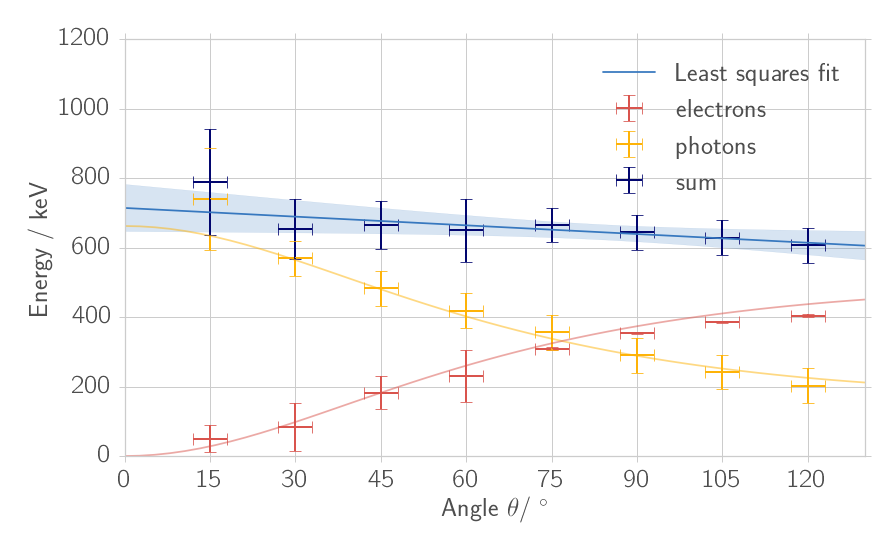
\includegraphics[width=0.9\linewidth]{./analysis/figures/energy_conservation}
    \caption{Summary of the analysis of the foregoing chapter. We note several aspects:
    The errors at small angles for the photon energies are rather high. 
    As result their weight in the fit will
    be rather small. Furthermore we arrive at a small tendency of a negative slope, which
    would disagree with energy conservation. However, this tendency is small, it is
    $[-0.7 \pm 0.8]$ keV/$^\circ$ where the height is $[750 \pm 80]$keV.}
\label{fig:energy_conservation}
\end{figure}

